\documentclass{article}

\usepackage{graphicx}
\usepackage{tikz}
\usepackage{tikzsymbols}
\usetikzlibrary{calc,patterns,shapes.geometric}
\pagestyle{empty}
\usepackage[margin=0pt]{geometry}
\geometry{papersize={14in,12in}}

\def\centerarc[#1](#2)(#3:#4:#5){\draw[#1] ($(#2)+({#5*cos(#3)},{#5*sin(#3)})$) arc (#3:#4:#5);}

\begin{document}
	\begin{figure}
		\centering
		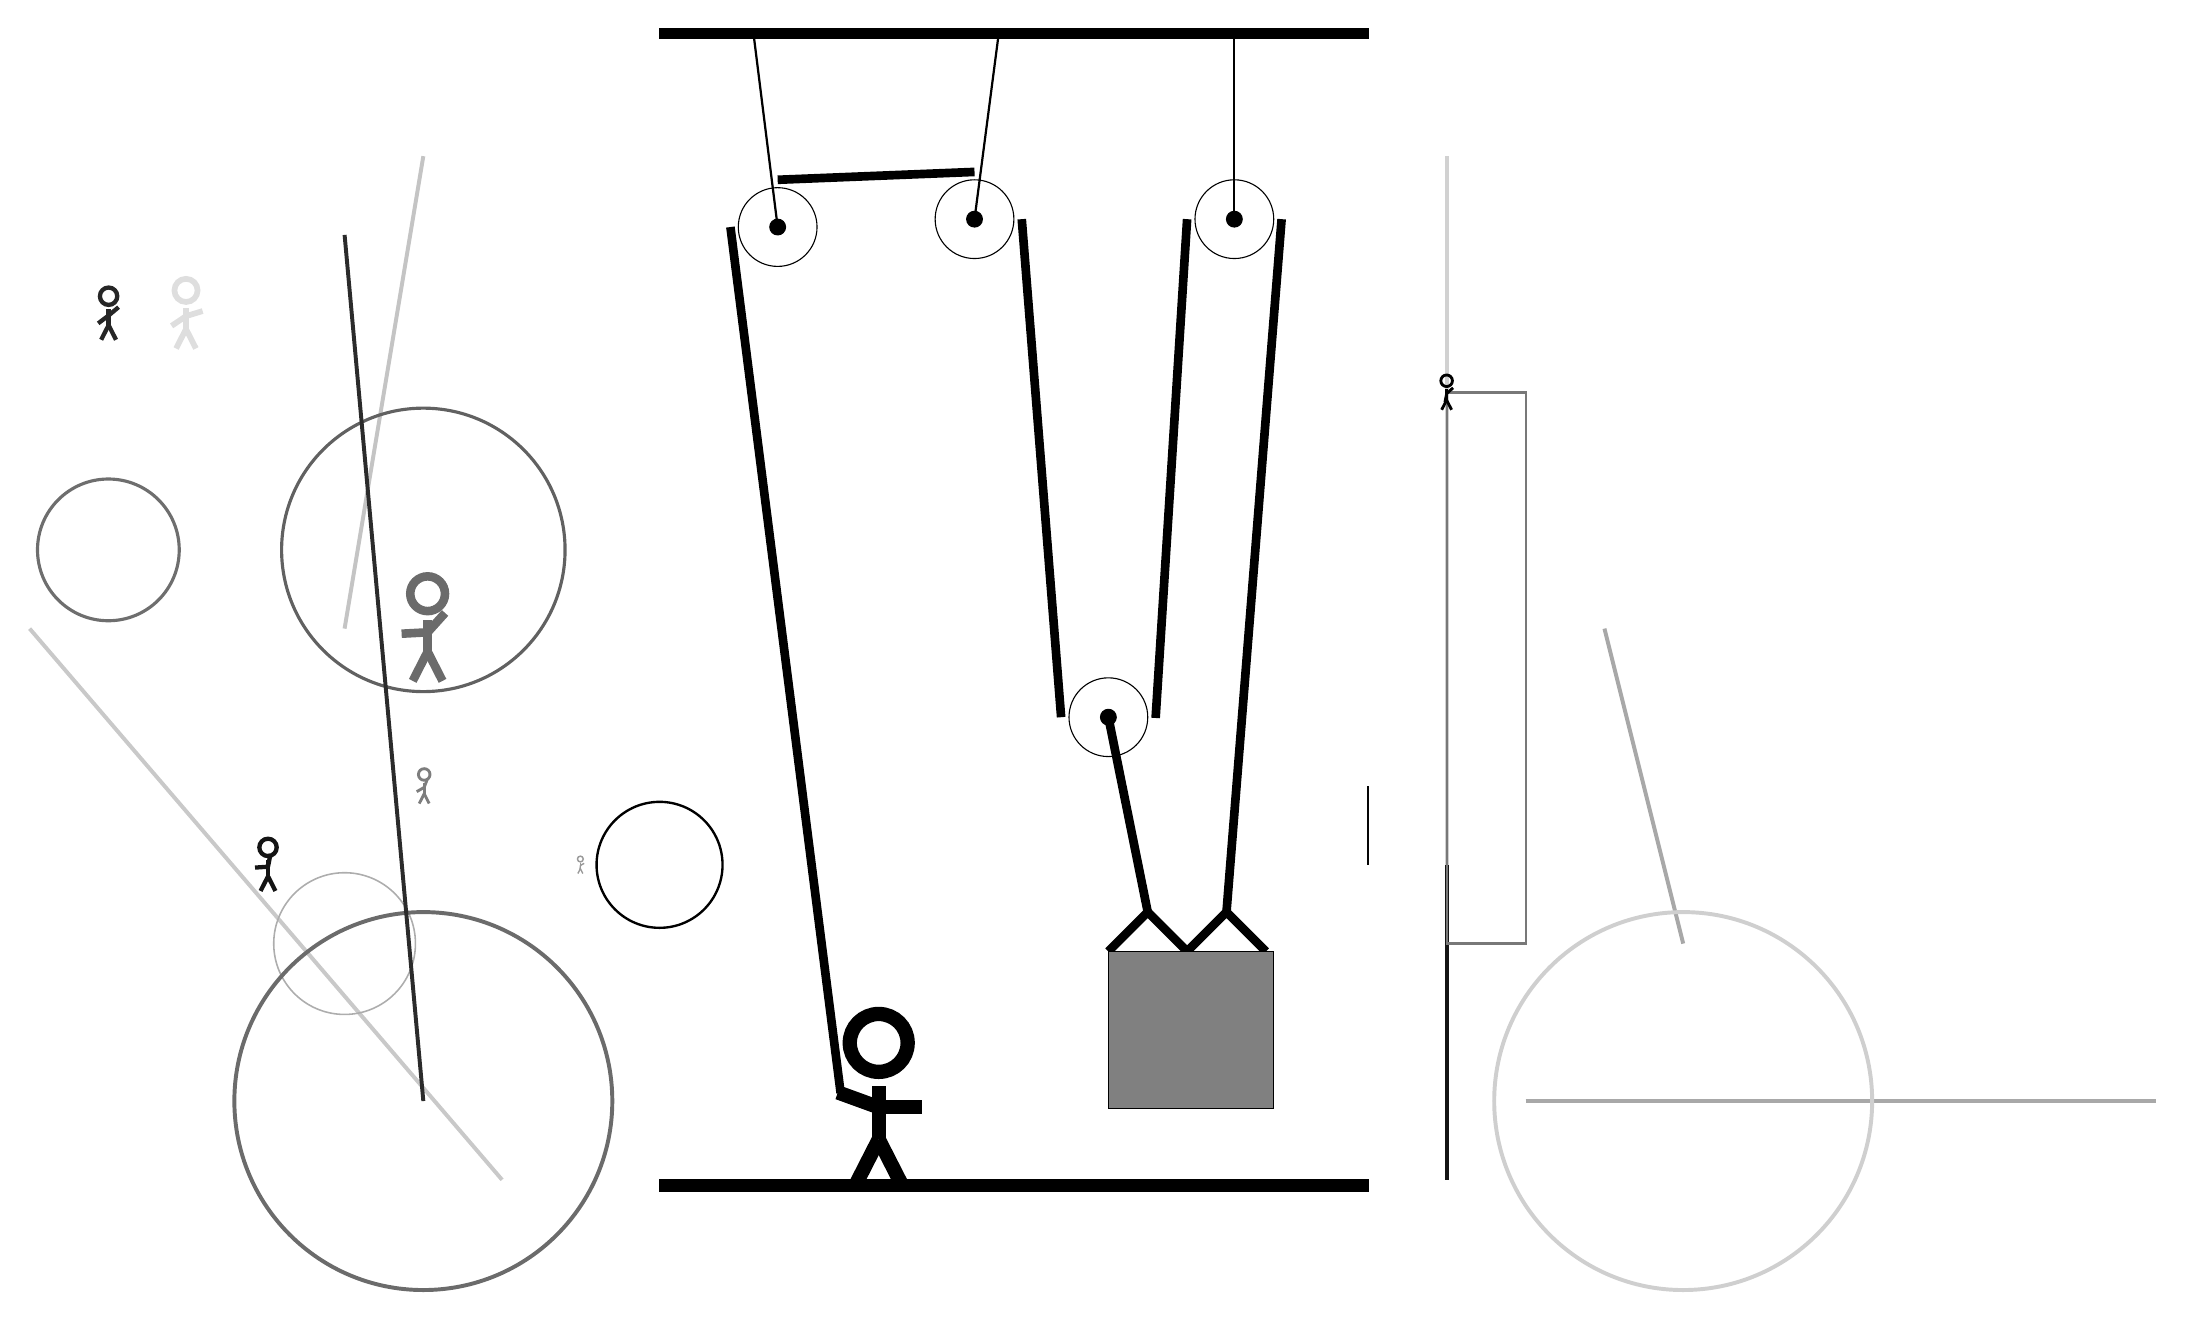
\begin{tikzpicture}
			%%%%% START %%%%%
			
			\draw[fill=black] (-3, 11.5) rectangle (6, 11.625);
			
			\draw (1, 9.2) circle (0.5);
			\draw[fill=black] (1, 9.2) circle (0.1);
			\draw[thick] (1, 9.2) -- (1.3, 11.5);
			
			\draw (4.3, 9.2) circle (0.5);
			\draw[fill=black] (4.3, 9.2) circle (0.1);
			\draw[thick] (4.3, 9.2) -- (4.3, 11.5);
			
			\draw (2.7, 2.875) circle (0.5);
			\draw[fill=black] (2.7, 2.875) circle (0.1);
			
			\draw[line width=1.1mm]  (2.7, -0.1) -- (3.2, 0.4) -- (3.7, -0.1) -- (4.2, 0.4) -- (4.7, -0.1);
			\draw[fill=black!50] (2.7, -0.1) rectangle (4.8, -2.1);
			
			\draw (-1.5, 9.1) circle (0.5);
			\draw[fill=black] (-1.5, 9.1) circle (0.1);
			\draw[thick] (-1.5, 9.1) -- (-1.8, 11.5);
			
			\node[line width=0.5mm, color=black!13] at (-9, 8) {\Strichmaxerl[4][34][17]};
			
			\draw[line width=0.5mm, color=black!92] (7, -3) rectangle (7, 9);
			\draw[line width=0.5mm, color=black!21](-5, -3) -- (-11, 4);
			\draw [line width=0.4mm, color=black!57](-10, 5) circle (0.9);
			\draw[line width=0.5mm, color=black!34](8, -2) -- (16, -2);
			\node[line width=0.3mm, color=black!58] at (-6, 4) {\Strichmaxerl[6][3][48]};
			\draw[line width=0.5mm, color=black!23](-7, 4) -- (-6, 10);
			\draw[line width=0.2mm, color=black!98] (6, 1) rectangle (6, 2);
			\draw[line width=0.4mm, color=black!18] (7, 10) rectangle (7, 1);
			\node[line width=0.5mm, color=black!40] at (-4, 1) {\Strichmaxerl[1][86][29]};
			\node[line width=0.6mm, color=black!51] at (-6, 2) {\Strichmaxerl[2][30][69]};
			\draw[line width=0.5mm, color=black!34](10, 0) -- (9, 4);
			\draw [line width=0.2mm, color=black!32](-7, 0) circle (0.9);
			
			\draw[line width=0.3mm, color=black!53] (8, 0) rectangle (7, 7);
			\draw [line width=0.5mm, color=black!58](-6, -2) circle (2.4);
			\node[line width=0.7mm, color=black!92] at (-8, 1) {\Strichmaxerl[3][4][79]};
			
			\draw [line width=0.4mm, color=black!62](-6, 5) circle (1.8);
			
			\node[line width=0.7mm, color=black!85] at (-10, 8) {\Strichmaxerl[3][37][40]};
			\node[line width=0.5mm, color=black!100] at (7, 7) {\Strichmaxerl[2][79][42]};
			\draw [line width=0.3mm, color=black!100](-3, 1) circle (0.8);
			\draw[line width=0.5mm, color=black!83](-7, 9) -- (-6, -2);
			
			\draw [line width=0.5mm, color=black!19](10, -2) circle (2.4);
			
			\draw[line width=1.1mm](-0.7, -1.9) --  (-2.1, 9.1);
			\centerarc[line width=1.1mm](-1.5, 9.1)(90:180:0.6);
			\draw[line width=1.1mm](-1.5, 9.7) -- (1, 9.8);
			\centerarc[line width=1.1mm](1, 9.2)(0:90:0.6);
			\draw[line width=1.1mm](1.6, 9.2) -- (2.1, 2.875);
			\centerarc[line width=1.1mm](2.7, 2.875)(180:370:0.6);
			\draw[line width=1.1mm] (3.3, 2.865) -- (3.7, 9.2);
			\centerarc[line width=1.1mm](4.3, 9.2)(0:180:0.6);
			\draw[line width=1.1mm](4.2, 0.4) -- (4.9, 9.2);
			\draw[line width=1.1mm] (3.2, 0.4) -- (2.7, 2.875);
			
			\node at (-0.2, -2) {\Strichmaxerl[10][-20][0]};
			
			\draw[fill=black] (-3, -3) rectangle (6, -3.15);
			
			%%%%% END %%%%%
		\end{tikzpicture}
	\end{figure}	
\end{document}